\section{Resultados e Discussões}
\label{sec-resultados}

Os modelos foram avaliados utilizando os nove sabores classificados como estabelecidos (Seção \ref{sec-materiais}.1). Na regressão linear, foram utilizadas 108 instâncias para treinamento e 27 para teste. Para a LSTM, empregaram-se 81 sequências de treinamento e 27 de teste, em decorrência da utilização de janelas temporais de três meses (\textit{lookback} = 3).

\subsection{Regressão Linear}

A Tabela \ref{tab:predlinear} apresenta os valores de $R^2$ obtidos pela regressão linear para cada sabor nos conjuntos de treinamento e teste.

\begin{table}[htpb]
\centering
\caption{Regressão Linear - R² por sabor}
\label{tab:predlinear} 
\begin{tabular} {cp{3.6cm}cc} \hline
\textbf{ID}&\textbf{Sabor} & \textbf{R² (Treino, N = 12)} & \textbf{R² (Teste, N = 3)} \\ \hline
1&Abacaxi & 0,232 & -7,271\\ 
2&Abacaxi com Hortelã & 	0,228 & -0,007\\ 
3&Bergamota & -0,020 & -0,371\\ 
6&Laranja & 0,470 & -15,952\\ 
7&Laranja e Couve & 0,066 & -2,410\\ 
9&Limonada & 0,422 & 0,590\\ 
10&Maracujá & -0,021 & -7,111\\ 
13&Morango & 0,410 & 0,405\\ 
15&Uva & -0,066 & 0,150\\ \hline
&\textbf{Global} & 0,921 & \textbf{0,897}\\\hline
\end{tabular}
\end{table}
\vspace{5em}
Apesar do elevado valor de $R^2$ global obtido no conjunto de teste (0,897), sua interpretação requer cautela, pois a métrica é sensível às diferenças de escala existentes entre os sabores avaliados. Considerando o $R^2$ por sabor, adotado como principal métrica de avaliação, observa-se desempenho heterogêneo. Os sabores Limonada ($R^2=0,590$), Morango ($R^2=0,405$) e Uva ($R^2=0,150$) apresentaram desempenho satisfatório, enquanto Abacaxi, Laranja e Maracujá obtiveram valores negativos. O pior resultado foi observado para o sabor Laranja ($R^2=-15,952$). Apesar da correção de inconsistências identificadas na base de dados, a elevada variabilidade da série histórica desse sabor (coeficiente de variação de 26,5\%) e o reduzido número de observações no conjunto de teste contribuíram para a instabilidade do coeficiente de determinação.

A análise dos coeficientes do modelo indica que as variáveis temperatura ($+0{,}21$) e mês de referência ($+0{,}28$, na representação cíclica) estão positivamente associadas ao volume de vendas, corroborando a influência da sazonalidade discutida na Seção \ref{sec-introducao}. As variáveis autorregressivas volume do mês anterior ($+1{,}43$) e média móvel de três meses ($-0{,}68$) apresentaram sinais opostos, comportamento compatível com a elevada correlação entre ambas e característico de multicolinearidade. Por fim, o coeficiente associado ao identificador do sabor ($-0{,}05$) apresentou baixa magnitude, resultado esperado devido à representação numérica adotada para uma variável originalmente categórica.

\begin{figure}[htpb]
    \centering
    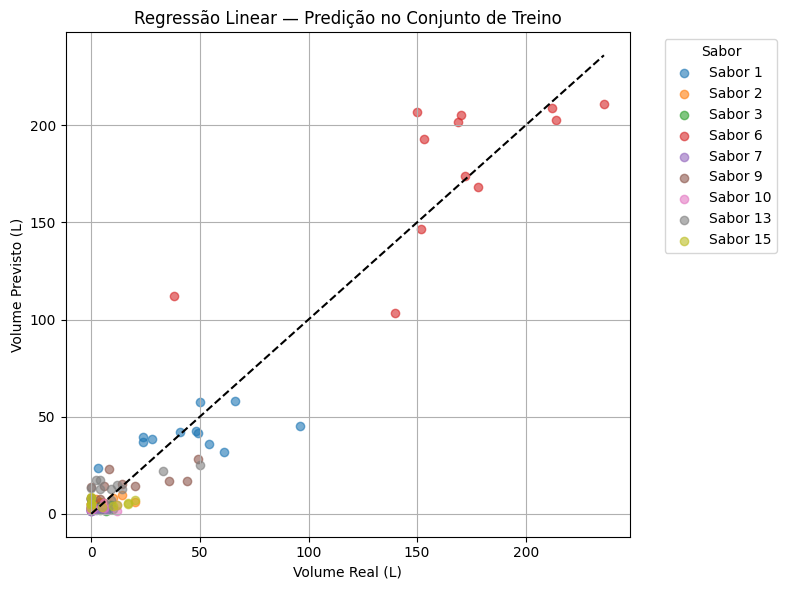
\includegraphics[width=0.5\linewidth]{imagens/Linear/RLTreino.png}
    \caption{Predições no conjunto de treinamento de OLS. Fonte: Autores (2026)}
    \label{fig:OLStrain}
\end{figure}

\begin{figure}[htpb]
    \centering
    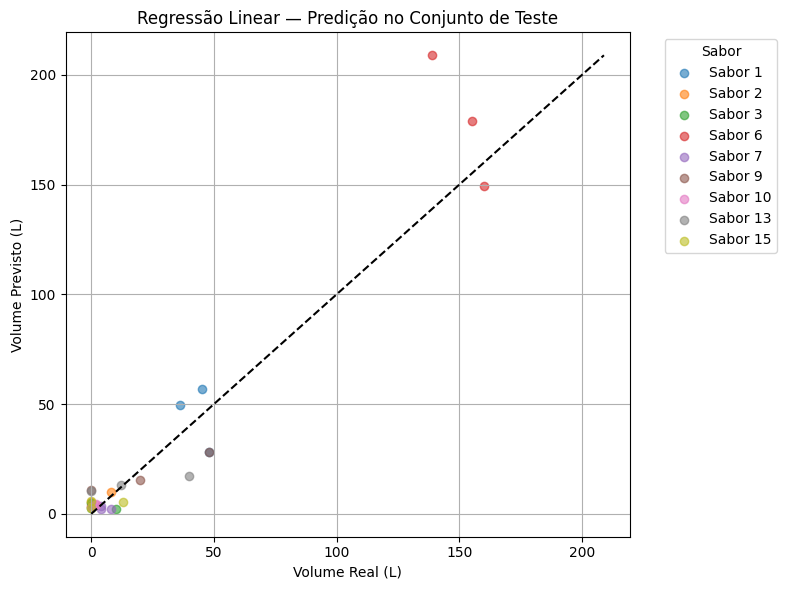
\includegraphics[width=0.5\linewidth]{imagens/Linear/RLTeste.png}
    \caption{Predições no conjunto de teste de OLS. Fonte: Autores (2026)}
    \label{fig:OLStest}
\end{figure}

As Figuras \ref{fig:OLStrain} e \ref{fig:OLStest} ilustram a dispersão entre os valores previstos e observados nos conjuntos de treinamento e teste, respectivamente. Observa-se maior concentração de pontos próximos à linha de identidade nos sabores de menor
volume, enquanto os sabores de maior escala exibem maior dispersão em torno dessa linha, refletindo a variabilidade absoluta mais elevada desses produtos.

\subsection{LSTM}

\begin{table} [htpb]
\centering
\caption{LSTM - R² por sabor}
\label{tab:predlstm} 
\begin{tabular} {cp{3.6cm}cc} \hline
\textbf{ID} & \textbf{Sabor} & \textbf{R² (Treino, N = 9)} & \textbf{R² (Teste, N = 3)} \\ \hline
1& Abacaxi & 	-0,488 & -0,125\\ 
2& Abacaxi com Hortelã & 	-0,319 & -0,366\\ 
3&Bergamota & -2,294 & -0,500\\ 
6&Laranja & -0,110 & -42,985\\ 
7&Laranja e Couve & 	-1,272 & -0,962\\ 
9&Limonada & 0,349 & 0,713\\ 
10&Maracujá & -3,321 & -0,635\\ 
13&Morango & 0,015 & -1,755\\ 
15&Uva & 	-0,618 & -0,277\\ \hline
&\textbf{Global} & 0,927 & \textbf{0,975}\\\hline
\end{tabular}
\end{table}
\vspace{1em}

A Tabela \ref{tab:predlstm} apresenta os resultados obtidos pela rede LSTM. Assim como na regressão linear, o $R^2$ global permaneceu elevado (0,975 no conjunto de teste), enquanto a avaliação individual por sabor revelou desempenho significativamente inferior. Com exceção da Limonada, que apresentou $R^2$ positivo tanto no treinamento (0,349) quanto no teste (0,713), todos os demais sabores obtiveram desempenho negativo no conjunto de teste. Esse foi também o único caso em que a LSTM superou a regressão linear. 

O sabor Laranja apresentou novamente o menor desempenho ($R^2=-42,985$), indicando que a arquitetura recorrente não foi capaz de modelar adequadamente sua elevada variabilidade com apenas nove sequências de treinamento.

\begin{figure} [htpb]
    \centering
    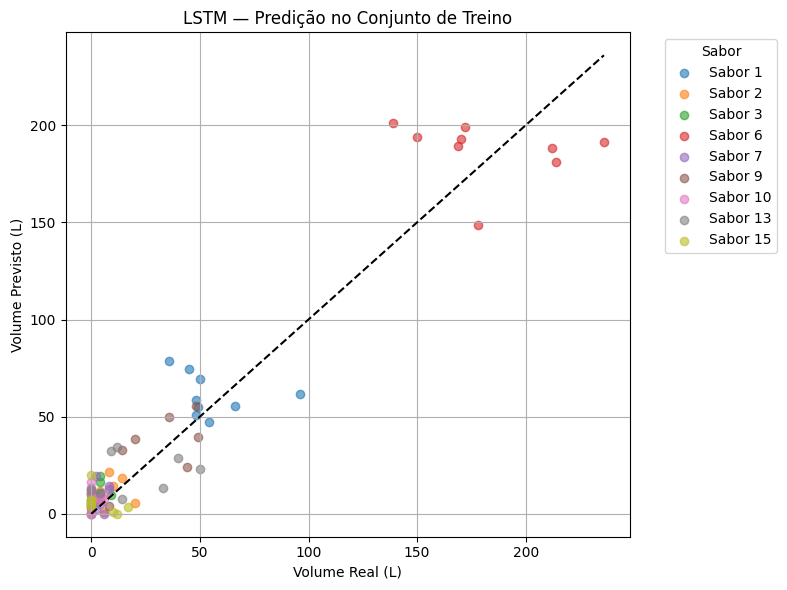
\includegraphics[width=0.5\linewidth]{imagens/LSTM/LSTMTreino.png}
    \caption{Correlação do modelo de treino de LSTM. Fonte: Autores (2026)}
    \label{fig:LSTMtrain}
\end{figure}
\vspace{1em}
\begin{figure} [htpb]
    \centering
    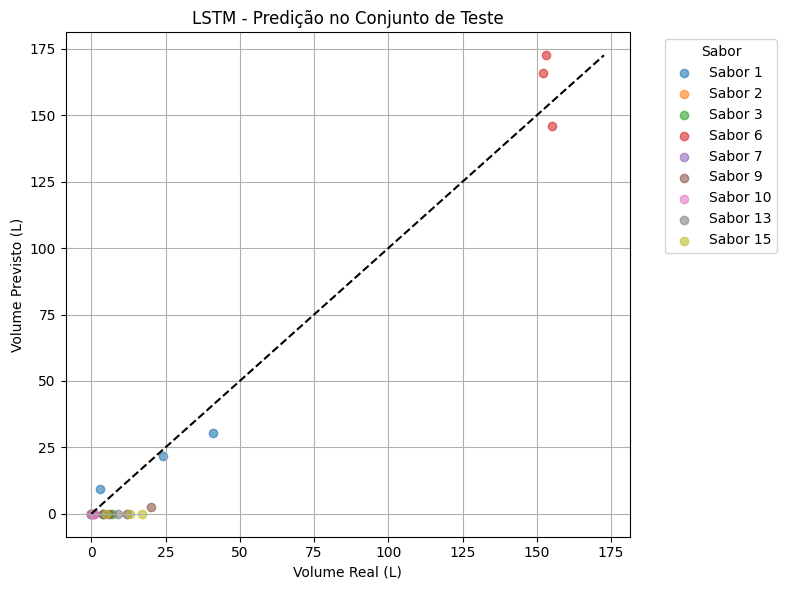
\includegraphics[width=0.5\linewidth]{imagens/LSTM/LSTMTeste.png}
    \caption{Correlação do modelo de teste de LSTM. Fonte: Autores (2026)}
    \label{fig:LSTMtest}
\end{figure}     

As Figuras \ref{fig:LSTMtrain} e \ref{fig:LSTMtest} apresentam os resultados obtidos para o modelo LSTM. Em comparação com a regressão linear, apresentados nas Figuras \ref{fig:OLStrain} e \ref{fig:OLStest}, observa-se maior dispersão entre os valores previstos e observados, especialmente no conjunto de teste, comportamento compatível com os valores de $R^2$ predominantemente negativos apresentados na Tabela \ref{tab:predlstm}.

A Figura \ref{fig:validation} apresenta a evolução do erro quadrático médio (MSE) ao longo das 200 épocas de treinamento do modelo LSTM, para os conjuntos de treinamento e de validação interna. Observa-se redução acentuada do erro nas primeiras 25 épocas, seguida de convergência gradual até a estabilização, a partir de aproximadamente 75 épocas, em um patamar próximo de zero em escala normalizada. A curva de validação estabiliza-se em valores ligeiramente inferiores à curva de treinamento ao longo da maior parte do processo, sem indícios de divergência crescente entre as duas curvas  o que descarta sobreajuste (\textit{overfitting}) progressivo como explicação para o baixo desempenho da LSTM no conjunto de teste, reforçando a interpretação já discutida na Seção \ref{sec-resultados}.1 de que a limitação decorre predominantemente do volume insuficiente de dados por sabor, e não de treinamento excessivo.

\begin{figure}[htpb]
    \centering
        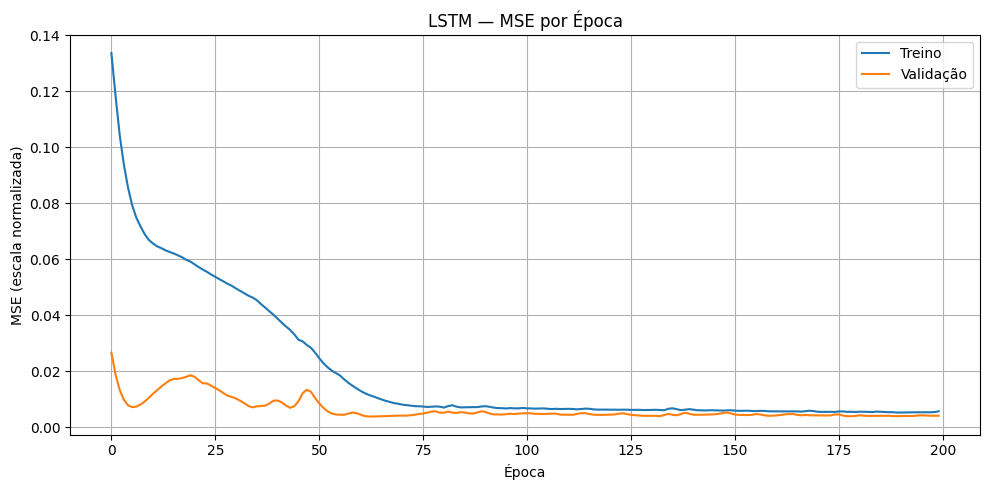
\includegraphics[width=0.8\linewidth]{imagens/LSTM/LSTMMSE.png}
    \caption{Gráfico de MSE do modelo de LSTM. Fonte: Autores (2026)}
    \label{fig:validation}
\end{figure}


\subsection{Comparação entre os modelos}

Considerando o $R^2$ por sabor no conjunto de teste, a regressão linear apresentou desempenho superior ao da LSTM em oito dos nove sabores avaliados, sendo superada apenas para o sabor Limonada. De modo geral, a regressão linear produziu previsões mais próximas da variabilidade observada nos dados, enquanto a LSTM apresentou erros de maior magnitude, especialmente para sabores com maior variabilidade temporal.

Esse resultado está de acordo com a literatura, que indica que arquiteturas de aprendizado profundo tendem a demandar maior volume de dados para superar modelos estatísticos tradicionais \cite{veres2024application}. No presente estudo, cada sabor estabelecido dispõe de apenas nove a doze observações mensais para treinamento, quantidade insuficiente para explorar adequadamente a capacidade de generalização da LSTM. Nessas condições, a regressão linear mostrou-se mais robusta e consistente.

As Figuras \ref{fig:plot} e \ref{fig:boxplot} complementam essa análise ao apresentarem, respectivamente, a evolução temporal e a distribuição estatística do volume de vendas dos sabores estabelecidos. A Figura \ref{fig:plot} mostra que o sabor Laranja apresenta o maior volume médio de vendas, acompanhado de elevada variabilidade temporal, com oscilações entre valores próximos de 140 L e superiores a 200 L. Esse comportamento é confirmado pela Figura \ref{fig:boxplot}, na qual o sabor Laranja exibe a maior amplitude interquartil e dispersão, embora mantenha mediana superior à dos demais sabores. Em contraste, sabores de menor volume, como Bergamota, Maracuja e Laranja e Couve, apresentam baixa variabilidade absoluta e valores concentrados próximos de zero, ainda que ocorram outliers associados a períodos específicos de maior demanda, como o pico observado para o sabor Abacaxi em agosto de 2025 (Figura \ref{fig:plot}). A elevada variabilidade absoluta do sabor Laranja contribui para explicar seus menores valores de R², tanto na regressão linear quanto na LSTM (Tabelas \ref{tab:predlinear} e \ref{tab:predlstm}), uma vez que erros absolutos de previsão tendem a ser maiores em séries de maior magnitude, reduzindo o coeficiente de determinação, especialmente em conjuntos de teste de tamanho limitado.


\begin{figure}[htpb]
    \centering
        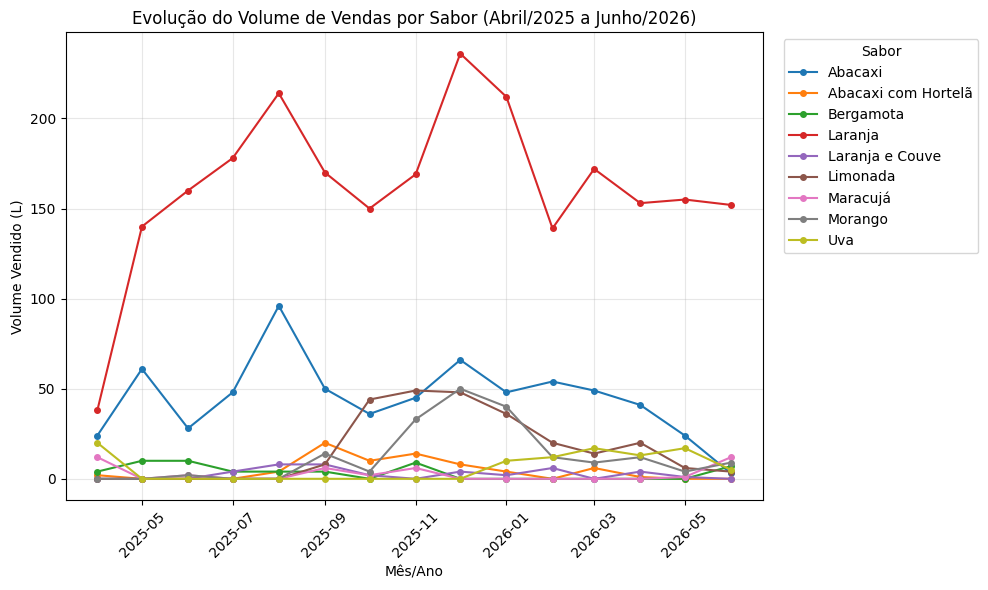
\includegraphics[width=0.8\linewidth]{imagens/Outros/plot.png}
    \caption{Gráfico de linhas de volume de vendas. Fonte: Autores (2026)}
    \label{fig:plot}
\end{figure}

\begin{figure}[htpb]
    \centering
        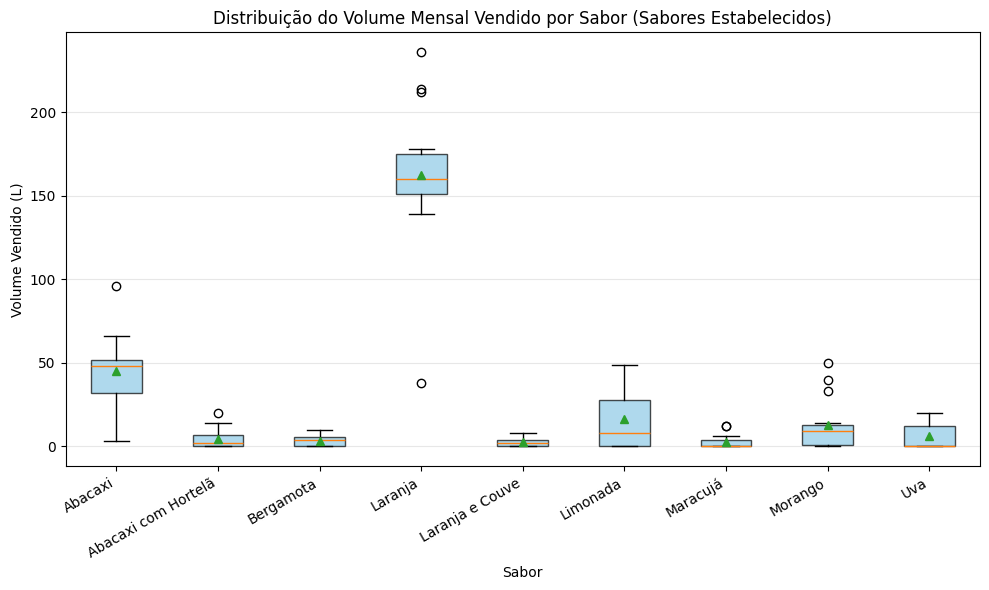
\includegraphics[width=0.78\linewidth]{imagens/Outros/boxplot.png}
    \caption{Gráfico de caixa de volume de vendas. Fonte: Autores (2026)}
    \label{fig:boxplot}
\end{figure}

\subsection{Previsão para Junho de 2026}

Para avaliar a aplicação prática dos modelos, ambos foram retreinados utilizando todas as observações disponíveis até maio de 2026, reservando junho de 2026 como conjunto de validação prospectiva (\textit{holdout}). A Tabela \ref{tab:predjun2026} apresenta as previsões obtidas.

\begin{table} [htpb]
\centering
\caption{Previsões para junho de 2026: valores reais vs. modelos}
\label{tab:predjun2026} 
\begin{tabular}{p{3.6cm}ccc} \hline
\textbf{Sabor} & \textbf{Real (L)} & \textbf{Regressão Linear (L)} & \textbf{LSTM (L)} \\ \hline
Abacaxi & 	3,0 & 32,8 & 	13,4\\ 
Abacaxi com Hortelã & 	0,0 & 1,4 & 0,0\\ 
Bergamota & 7,0 & 0,7 & 0,0\\  
Laranja & 152,0 & 152,7 & 154,3\\ 
Laranja e Couve & 	0,0 & 0,5 & 0,0\\ 
Limonada & 4,0 & 2,6 & 0,0\\ 
Maracujá & 12,0 & 0,7 & 0,0\\ 
Morango & 9,0 & 2,1 & 0,0\\ 
Uva & 	5,0 & 1,9 & 1,3\\ \hline
\end{tabular}
\end{table}

Os dois modelos apresentaram elevada precisão para o sabor Laranja, com previsões de 152,7 L e 154,3 L frente aos 152 L observados, correspondendo a erro relativo inferior a 2\%. Esse resultado é consistente com o fato de esse sabor possuir o maior histórico de vendas entre os analisados. Para os demais sabores, caracterizados por baixos volumes mensais de venda, as previsões apresentaram maior discrepância em relação aos valores observados. Destaca-se o caso do Abacaxi, cuja demanda caiu para apenas 3 L em junho de 2026, enquanto a regressão linear e a LSTM estimaram 32,8 L e 13,4 L, respectivamente. Como essa redução não possui precedentes na série histórica, ambos os modelos tenderam a reproduzir o comportamento médio observado nos meses anteriores. De forma geral, a LSTM apresentou comportamento mais conservador, prevendo volume igual a zero para seis dos nove sabores avaliados. A regressão linear, por sua vez, produziu estimativas distintas de zero para todos os sabores, refletindo maior sensibilidade às diferenças de demanda entre os produtos.

\subsection{Estratégias de Gestão de Estoque}

Como a regressão linear apresentou desempenho superior na comparação entre os modelos, suas previsões foram utilizadas para definir três estratégias de planejamento de estoque: Conservadora, Equilíbrio e Otimista. A faixa de incerteza foi estimada com base no erro histórico de previsão de cada sabor, obtido por validação cruzada leave-one-out (LOOCV), na qual cada observação mensal é utilizada, sucessivamente, como conjunto de teste e as demais como conjunto de treinamento. O desvio-padrão dos erros resultantes (Tabela \ref{tab:loocv}) foi adotado como medida da incerteza associada às previsões. A partir dessas margens, definem-se as três estratégias operacionais para um dado sabor $i$ e período $t$:

\[\textit{Conservadora}_i(t) = max(0, \hat{y}_i(t)-\sigma_i).\]

\[\textit{Equilíbrio}_i(t) = \hat{y}_i(t).\]

\[\textit{Otimista}_i(t)=\hat{y}_i(t) + \sigma_i.\]

em que $\hat{y}_i(t)$ representa a previsão pontual do modelo para o sabor $i$ no período $t$, e $\sigma_i$ corresponde ao desvio-padrão do erro obtido por validação cruzada. A Tabela \ref{tab:estrategias} apresenta a aplicação dessas estratégias às previsões para junho de 2026.

\begin{table}[htpb]
\centering
\caption{Erro de previsão por sabor via validação cruzada \textit{leave-one-out}}
\label{tab:loocv}
\begin{tabular}{lcc}
\hline
\textbf{Sabor} & \textbf{MAE (L)} & \textbf{Desvio-padrão do erro (L)} \\
\hline
Abacaxi              & 18,9 & 23,7 \\
Abacaxi com Hortelã  & 4,0  & 5,6  \\
Bergamota             & 3,4  & 3,9  \\
Laranja               & 44,9 & 49,6 \\
Laranja e Couve       & 2,3  & 2,8  \\
Limonada              & 12,1 & 14,4 \\
Maracujá              & 2,9  & 4,2  \\
Morango               & 9,9  & 12,9 \\
Uva                   & 6,6  & 7,6  \\
\hline
\end{tabular}
\end{table}



\begin{table}[h]
\centering
\caption{Estratégias de estoque para junho de 2026, com base na Tabela \ref{tab:predjun2026}}
\label{tab:estrategias}
\begin{tabular}{p{3.56cm}cccc}
\hline
\textbf{Sabor} & \textbf{Real (L)} & \textbf{Conservadora (L)} & \textbf{Equilíbrio (L)} & \textbf{Otimista (L)} \\
\hline
Abacaxi           & 3,0   & 9,1   & 32,8  & 56,5  \\
Abacaxi com Hortelã  & 0,0   & 0,0   & 1,4   & 7,0   \\
Bergamota             & 7,0   & 0,0   & 0,7   & 4,6   \\
Laranja               & 152,0 & 103,1 & 152,7 & 202,3 \\
Laranja e Couve       & 0,0   & 0,0   & 0,5   & 3,3   \\
Limonada              & 4,0   & 0,0   & 2,6   & 17,0  \\
Maracujá              & 12,0  & 0,0   & 0,7   & 4,9   \\
Morango               & 9,0   & 0,0   & 2,1   & 15,0  \\
Uva                   & 5,0   & 0,0   & 1,9   & 9,5   \\
\hline
\end{tabular}
\end{table}

Para o sabor Laranja, o valor observado (152 L) situou-se dentro do intervalo definido pelas estratégias Conservadora (103,1 L) e Otimista (202,3 L), enquanto a Estratégia de Equilíbrio praticamente coincidiu com o valor real (152,7 L). Esse resultado era esperado, uma vez que esse sabor dispõe do maior histórico de dados para treinamento.

Nos sabores de menor volume, cinco dos oito valores observados permaneceram dentro da faixa delimitada pelas estratégias Conservadora e Otimista, mesmo quando a previsão pontual apresentou erro significativo. A principal exceção foi o sabor Abacaxi, cuja queda abrupta de demanda não pôde ser antecipada pelo modelo, fazendo com que até mesmo a Estratégia Conservadora superestimasse o volume efetivamente vendido.

As três estratégias representam diferentes níveis de tolerância ao risco no planejamento de estoque. A Estratégia Conservadora prioriza a redução de desperdícios de insumos perecíveis, enquanto a Estratégia Otimista busca minimizar o risco de ruptura de estoque por meio de maior disponibilidade de produtos. A Estratégia de Equilíbrio corresponde à previsão pontual do modelo e é indicada para o planejamento operacional em condições normais, podendo as demais estratégias ser utilizadas como limites inferior e superior de produção, conforme a política de gestão de riscos da empresa. Considerando que a empresa adota uma estratégia de demanda puxada, a Estratégia Conservadora mostra-se a mais compatível com seu contexto operacional.

Os resultados obtidos mostram que a complexidade do modelo não implica necessariamente melhor desempenho preditivo. Embora a LSTM seja capaz de representar relações temporais mais complexas, seu desempenho foi limitado pela pequena quantidade de dados disponível para cada sabor. Em contrapartida, a regressão linear apresentou maior capacidade de generalização, corroborando os achados de \cite{golabek2020demand} para produtos do setor de bebidas e reforçando a importância de selecionar modelos compatíveis com o volume e as características dos dados disponíveis.